\subsection{Neural Language Model}

In our computational experiments, we use a neural language model.
the Italian NLM made available by \citet{Gulordava:etal:2018} at \url{https://github.com/facebookresearch/colorlessgreenRNNs}.
Below we provide some details about this model and explain how it is trained and evaluated.

\begin{figure}
    \centering
    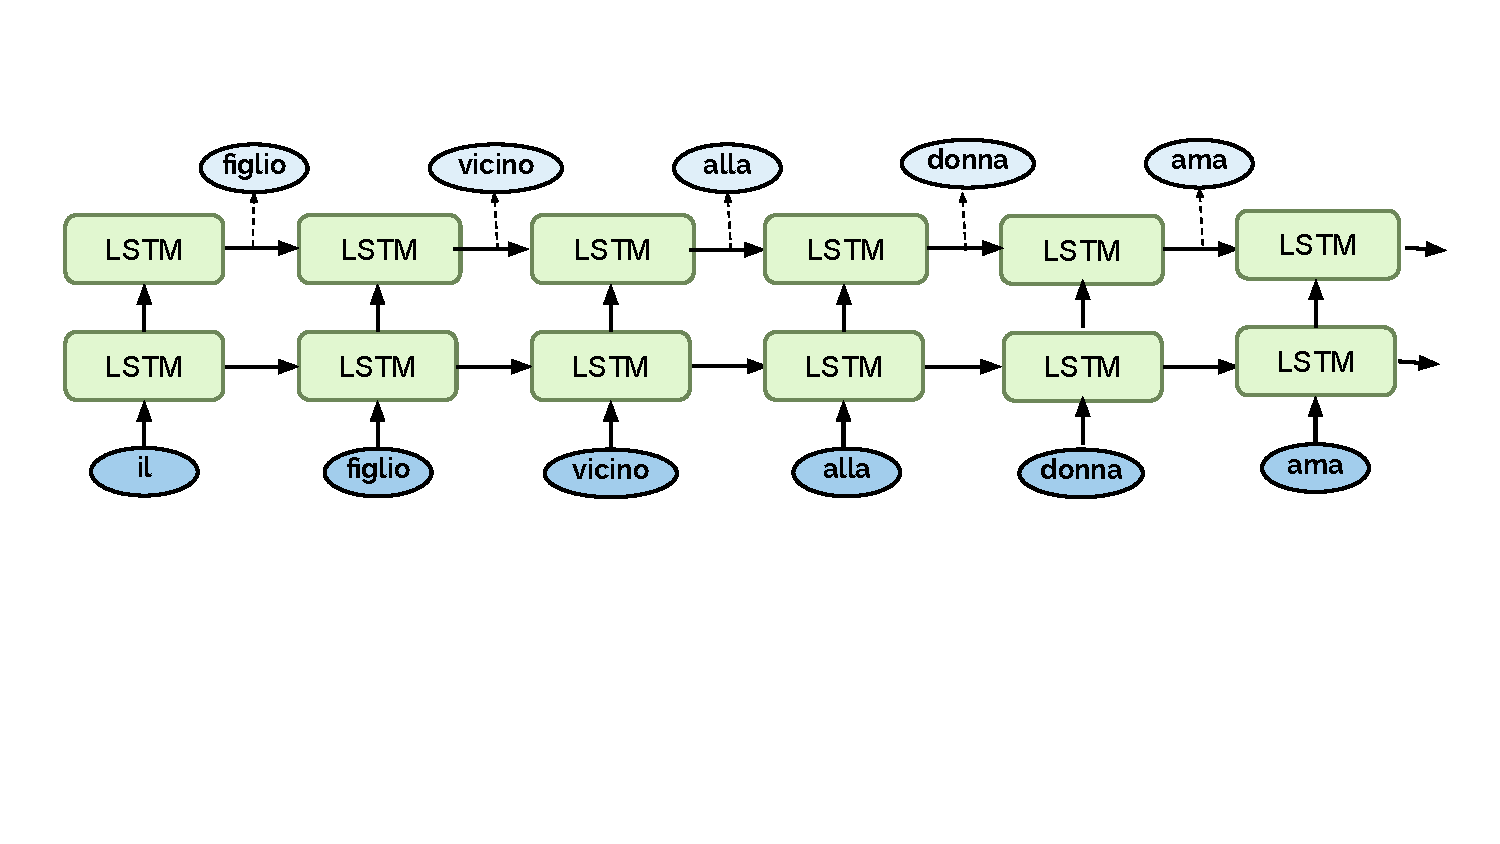
\includegraphics[width=0.8\textwidth, clip, trim={10mm 50mm 10mm 20mm}]{figures/LM-image}
    \caption{Graphical description of a two-layer LSTM language model. 
        At ever timestep, the model processes an input word and outputs a probability distribution over potential next words in the sentence.
    In our experiments, we do not consider the full probability distribution, but instead compare the probabilities of the relevant verbs and adjectives.
    \dieuwke{I am not very happy about this caption: it made me wonder whether the current depiction where no mention of probabilities is made is perhaps a bit too simple?}}
\end{figure}

\subsubsection{Model Description}
\dieuwke{@Yair: I could put some basic image if you want?}
The NLM we consider is a relatively basic \emph{recurrent} neural language model.
It consider of two layers with 650 Long-Short Term Memory (LSTM) units \citep{Hochreiter:Schmidhuber:1997}, input and output embedding layers of 650 units and input and output layers of size 50000 (the size of the vocabulary). The weights of the input and output embedding layers are not shared.
The last layer of the model is a softmax layer, whose activations sum up to 1 and as such corresponds to a probability distribution over all words in the NLM's vocabulary. 
The model was trained on a dump of the Italian Wikipedia (80M word token, 50K word types). 
Further details can by found in \citet{Gulordava:etal:2018}.

% \subsubsection{Control model Training} 
% \textbf{M: Given how little emphasis this has in the main text, how about moving it to supplementary? \dieuwke{Agree}} In addition to the NLM made available by \citet{Gulordava:etal:2018}, we train an additional 19 models using the same procedure and corpus (drawn from Wikipedia), giving 20 models in total. 
% The models differ in the order in which those sentences are presented as well as the initialization of their weights.
% For all runs, we use a learning rate of 20, a batch size of 64 and a dropout rate of 0.2, the hyperparameters that \citet{Gulordava:etal:2018} reported to work best for this particular corpus and setup.
% Following Gulordava, but contrary to common practice in language modeling, we train the models on separate sentences, rather than longer pieces of discourse.
% As common practice for training language models, we do not use an optimizer, but instead use a \emph{plateau-based} learning scheme, in which we half the learning rate whenever the validation perplexity of the model reaches a plateau.
% 
\subsubsection{NA-task evaluation Evaluation}
% After training, we evaluate the resulting 20 models by considering their perplexity on a shared test set\footnote{\url{https://dl.fbaipublicfiles.com/colorless-green-rnns/training-data/Italian/test.txt}}. 
Following \citet{Linzen:etal:2016}, we compute the model's accuracy for the different NA-tasks by considering whether the model prefers the correct verb or adjective form (for the NounPP and NounPP-gender tasks, respectively).
We do so by presenting the preamble of each sentence to the NLM and then comparing the output probabilities assigned to the plural and singular forms of the verb for the NounPP task and the probabilities of the masculine and feminine forms for the NounPP-gender task.
On each sentence, the model is scored 1 if the probability of the correct verb is higher than the wrong, and else 0. 
The model's accuracy is then defined as the average of these scores across all sentences in the NA-task. 

\subsubsection{Ablation Experiments}
To identify units that play an important role in the encoding of number and gender, we run a series of ablation tests.
In these ablation tests, we assess the impact of a \emph{single unit} on model performance by setting the activation of the unit to zero and then recomputing the performance of the model on the NounPP and NounPP-gender NA-tasks. 
We conduct such ablation studies for all recurrent units in the network, resulting in 1300 ablation studies per task.

